\documentclass[12pt,a4paper]{article}
\usepackage[margin=1in]{geometry}
\usepackage[utf8]{inputenc}
\usepackage[backend=biber,style=apa]{biblatex}
\usepackage{graphicx}
\usepackage{caption}
\usepackage[none]{hyphenat}
\usepackage{hyperref}
\usepackage[nameinlink]{cleveref}

\setlength{\fboxrule}{2pt}
\addbibresource{references.bib}
\setlength\bibitemsep{1.5\itemsep}
\defbibheading{bibempty}{}


\begin{document}
	\begin{titlepage}
		
		\begin{center}
			
\includegraphics[width=0.5\textwidth]{QUT.jpg}\\
			[0.03\textheight]  
			\Large\textbf{Bachelor of IT (Computer Science)}\\
			\Large\textbf{Assignment 2 - Creative Coding Project}\\
			\large\textbf{DXB211 - Creative Coding}\\
			[0.02\textheight]
			\large\textsl{Dane Madsen}\\
			\large\textsl{n10983864@qut.edu.au}
		\end{center}
		
	\end{titlepage}
	\tableofcontents
	\newpage

	\section{Introduction}
		In WWII Germany, Enigma was an instrumental tool in the German war effort. 
		Enigma was a machine used to encrypt and decrypt intelligence communications 
		between German forces. The sketch created for this assignment aims to simulate 
		the Enigma machines encryption and decryption process.\\
		\\
		To run this sketch you will need to run \texttt{python -m http.server} in the 
		\texttt{src} folder of the project. Then navigate to \texttt{localhost:8000} 
		in your web browser and open the \texttt{entry.html} file.\\
		\\
		To use the sketch, set the three rotors to the desired positions, then simply 
		type and plain text will be displayed next to the \texttt{Plain Text} heading along 
		with the encrypted / decrypted text next to the \texttt{Cipher Text} heading.\\

		\begin{center}
			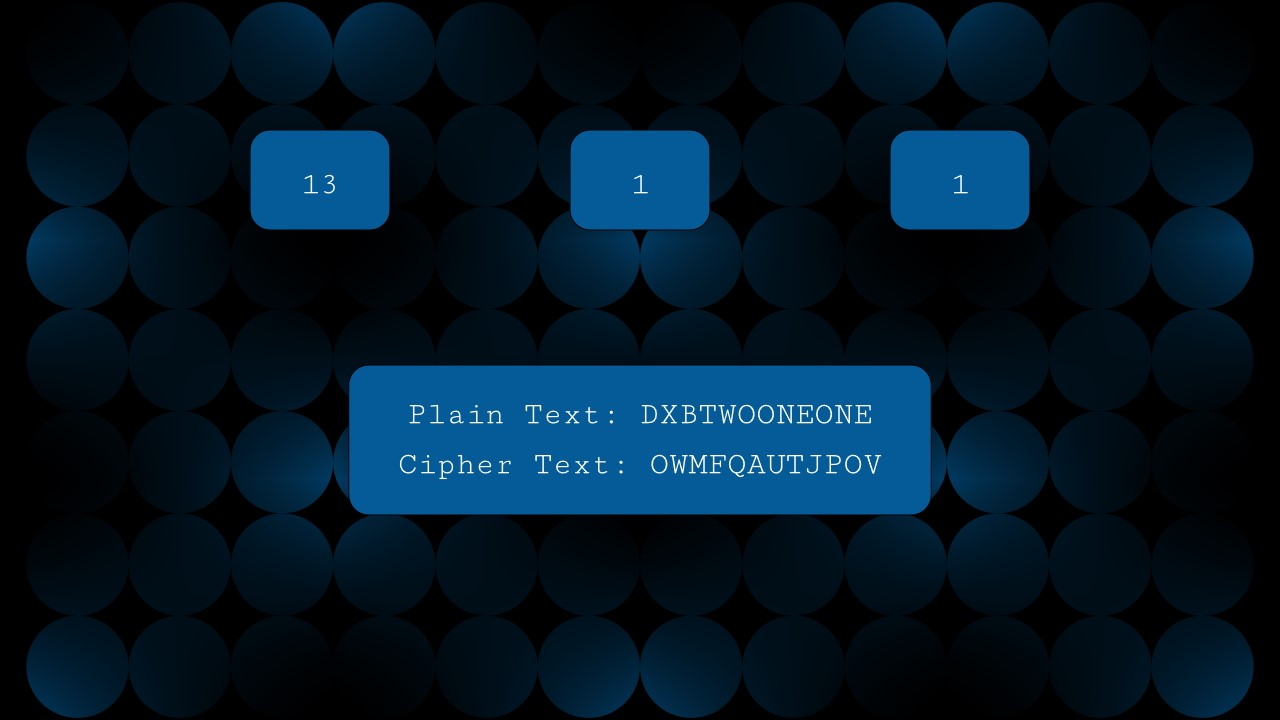
\includegraphics[width=0.8\textwidth]{figures/figure1.jpg}\\
			\vspace{0.5cm}
			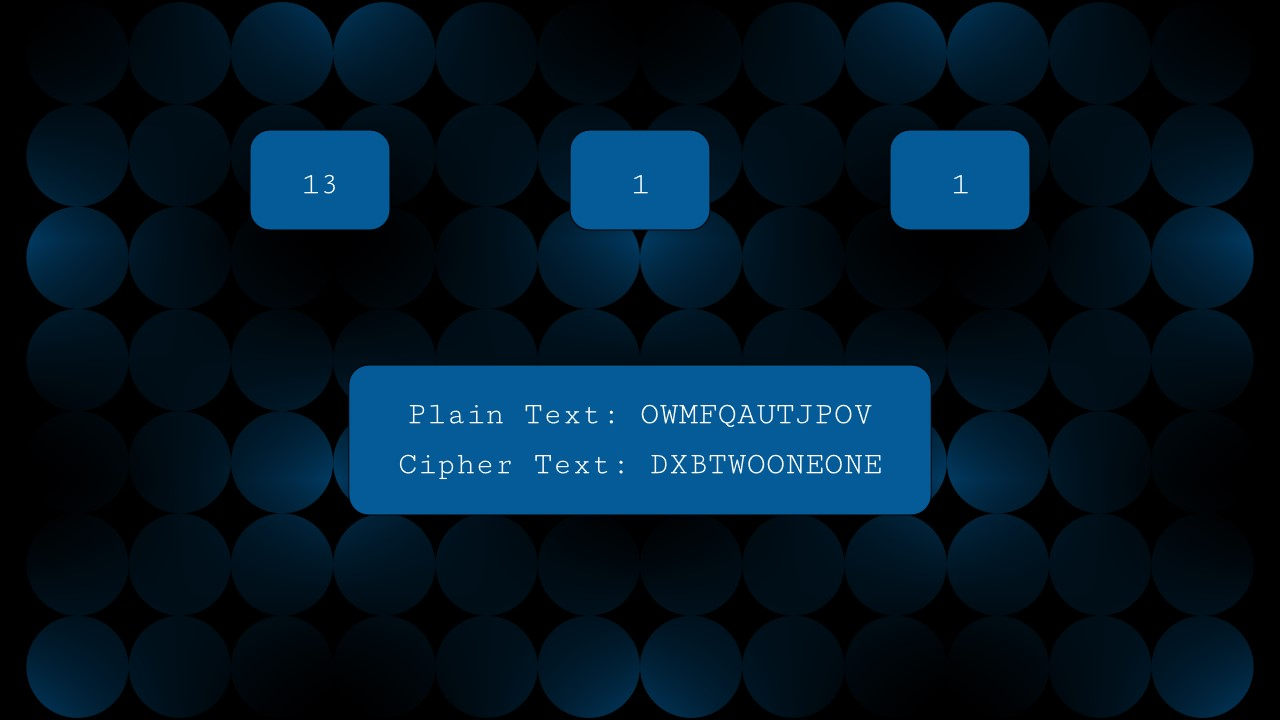
\includegraphics[width=0.8\textwidth]{figures/figure2.jpg}\\
		\end{center}
	
	\newpage

	\section{Design and Aesthetic}
		I chose to design a P5JS Enigma machine because I have always been interested 
		in Cryptography and the cabinets in the brief reminded me of the Enigma machine. 
		As such, creating a P5JS Enigma machine presented me with an opportunity to 
		both learn more about cryptography whilst also creating an interesting and appealing 
		sketch. I chose rounded boxes for the UI because I thought it made the sketch look 
		more modern and visually appealing.\\
		\\
		I used alot of blue in the sketch because I felt it evoked a sense of secrecy and 
		security which is what the Enigma machine was all about. One thing to note about the 
		function of the sketch is that the space key does not work when typing a message, 
		\textbf{this is intentional}. I chose to do it this way to maintain authenticity 
		with the real Enigma machine. The patten used as the background of my sketch is ment 
		to be roughly similar to a patten used on the \textcite{ASD2023} website. The reason 
		i chose Cutive Mono as the font is i thought it looked militaristic and fit the 
		theme of the sketch.\\

	\section{Design Process}
		In the initial design of the sketch, I planned to have the rotors displayed stacked 
		vertically in the center of the page. In this version of the sketch the actual values 
		of the rotors would be displayed accross the page as strings of text and the user could
		only advance the rotor by clicking on it. There was not any way for the user to reverse 
		the rotor at this point in time.\\

		\begin{center}
			\fbox{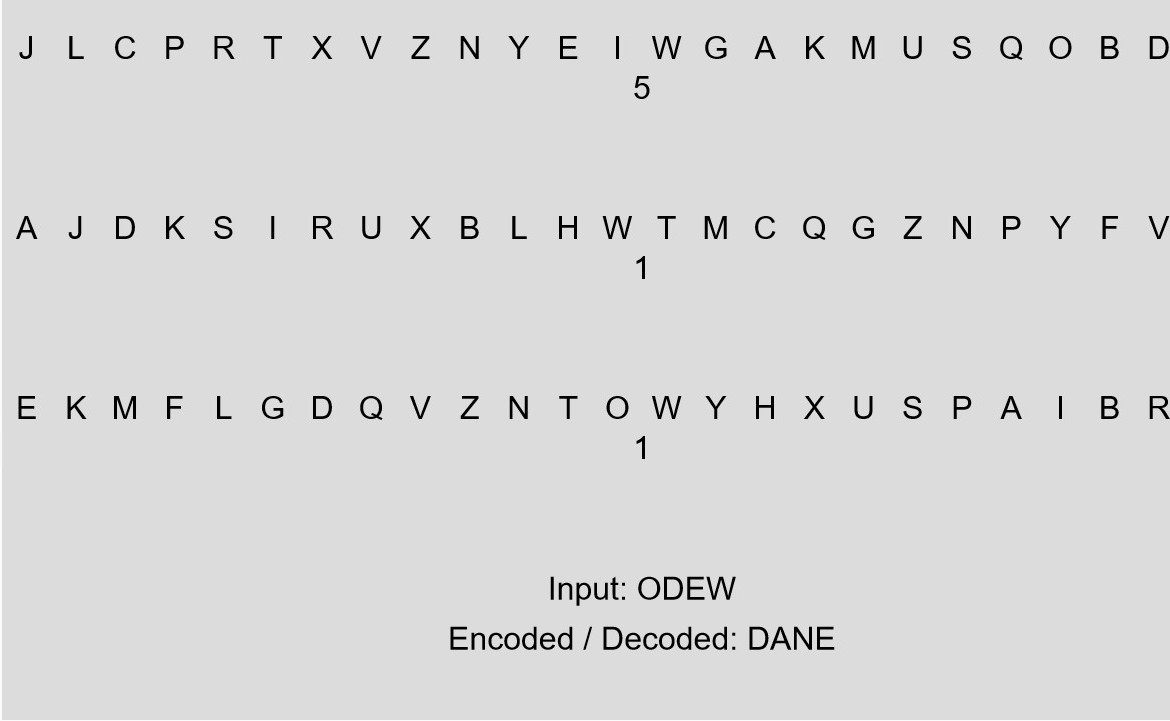
\includegraphics[width=0.8\textwidth]{figures/figure5.jpg}}\\
		\end{center}
		\newpage
		I thought this looked interesting but ultimately it served no purpose so I decided to 
		remove it in favor of a more minimalistic design with a simple number to represent 
		each rotor position. At this point I also took the liberty to chnage the arrangement of 
		the rotor position numbers to be side by side at the top of the page.\\
		
		\begin{center}
			\fbox{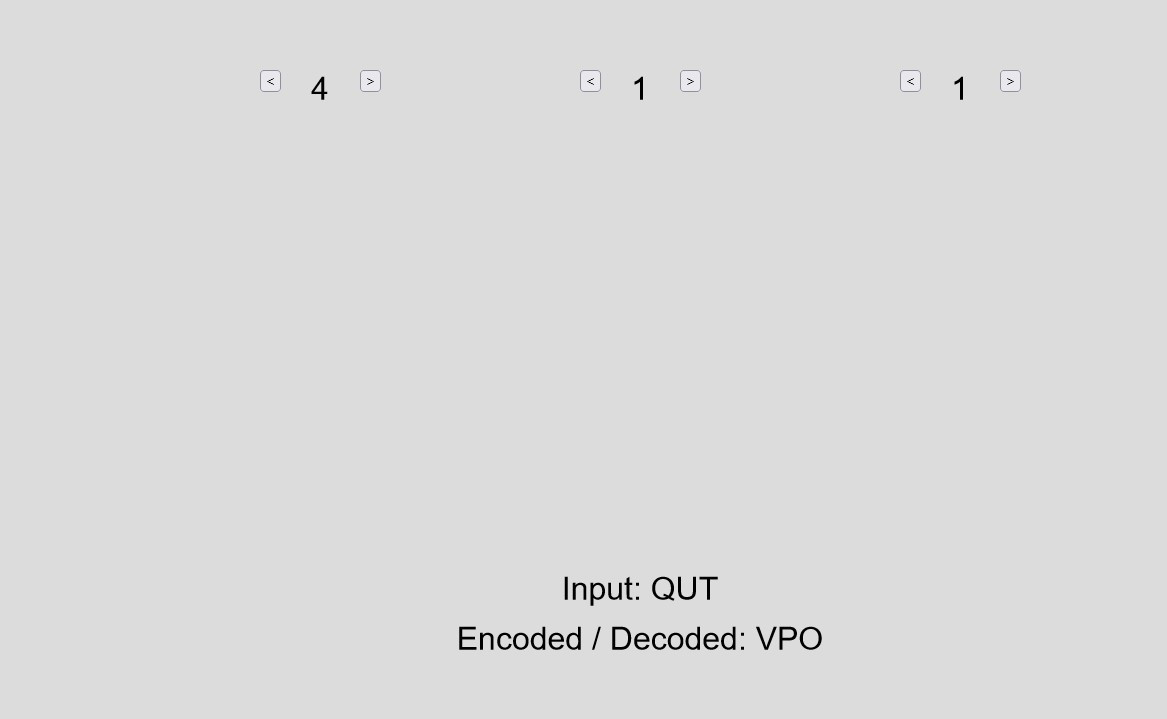
\includegraphics[width=0.8\textwidth]{figures/figure6.jpg}}\par
		\end{center}
		\vspace{0.5cm}
		Finally I settled on the design shown in the introduction. I decided to move the text 
		elements closer to the vertical center and added the background image and rounded squares 
		to make the sketch look more interesting. At this point the sketch looks very similar to the 
		final version with the only difference being the headings \texttt{Input} and 
		\texttt{Encoded / Decoded}.\\

		\begin{center}
			\fbox{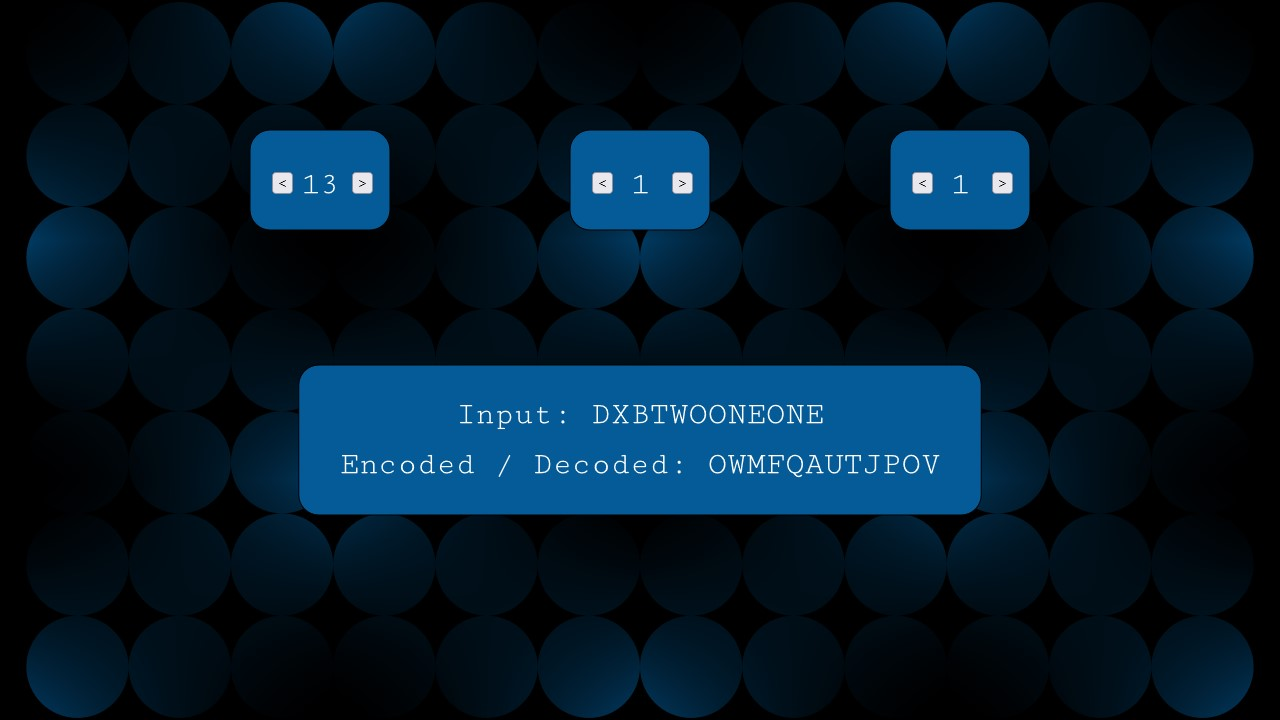
\includegraphics[width=0.8\textwidth]{figures/figure7.jpg}}\par
		\end{center}
	
	\newpage

	\section{Creative Influences}
		The sketch has been designed to roughly resemble the style of the 
		\textcite{ASD2023} website. The ASD is the intelligence agency of Australia responsible 
		for conducting signals intelligence on behalf of the Australian Government. As such, 
		Cryptography is highly relevant to the ASD's work. Another source of styling was 
		the website of \textcite{QUT2023}, which shared a similar color scheme to the ASD website.\\
		
		\begin{center}
			\fbox{
\includegraphics[width=0.8\textwidth]{figures/figure3.jpg}}\\
			\vspace{0.5cm}
			\fbox{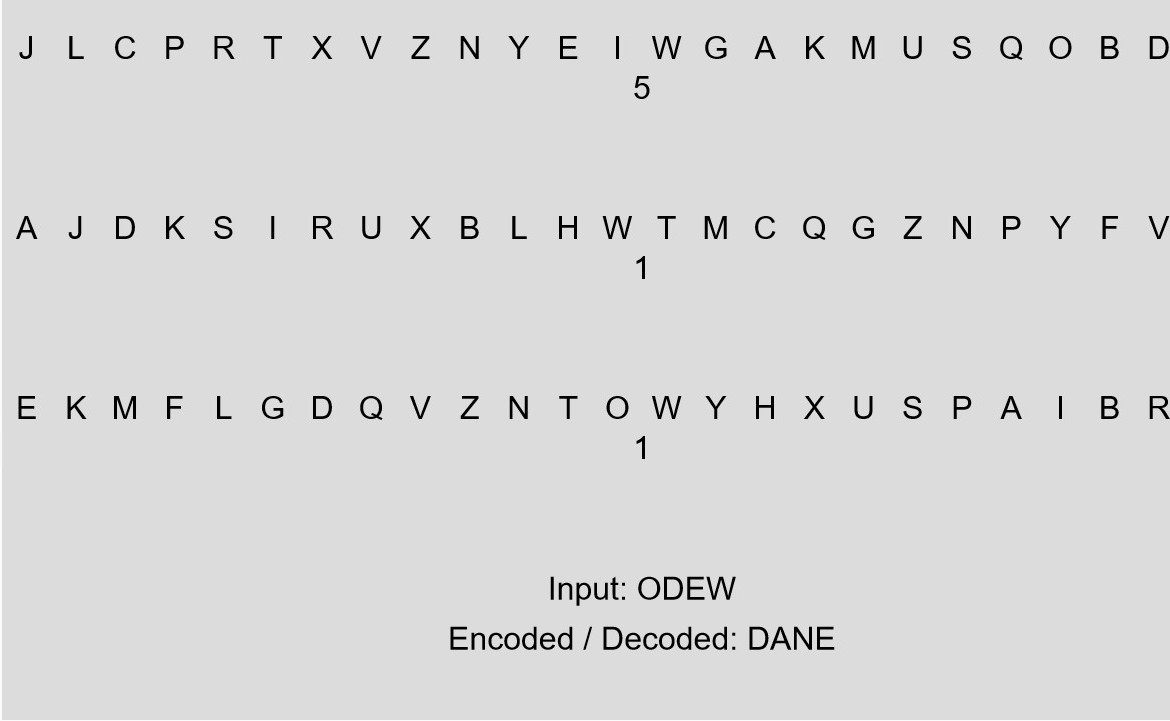
\includegraphics[width=0.8\textwidth]{figures/figure4.jpg}}\\
		\end{center}
		\vspace{0.5cm}
		The last influence of the sketch was the Enigma machine itself. For my sketch I used the same 
		number of rotors and reflector as the most common Enigma machine in WWII which I obtained from 
		a website called \textcite{CryptoMuseum2023}.
	
	\newpage

	\section{References}
	\printbibliography[heading=bibempty]

\end{document}